\documentclass{article}
\usepackage[a4paper, total={6.5in, 10in}]{geometry}
\usepackage{amsmath}
\usepackage{float}
\usepackage{enumitem}
\usepackage{graphicx}
\usepackage{hyperref}
\usepackage{diagbox}

\graphicspath{ {../Plots/} }

\setlength{\parindent}{0cm}

\title{Applied Data Science: Coursework Report}
\author{Daniel Petrov}
\date{24th December 2023}

\begin{document}

\maketitle
\tableofcontents

\newpage
\section{Section A}
The code used to produce the figures and answer the questions posed in this section are kept in the \verb|src/Q1.ipynb| file.
\subsection{Dataset A: Exploration, Dimensionality Reduction and Clustering}
\begin{enumerate}[label=\alph*)]
    \item The \verb|seaborn| package was used to produce density plots for the first 20 features of Dataset A. The plots are shown in Figure \ref{fig:Q1a_First20Features}.
    \begin{figure}[!htb]
        \centering
        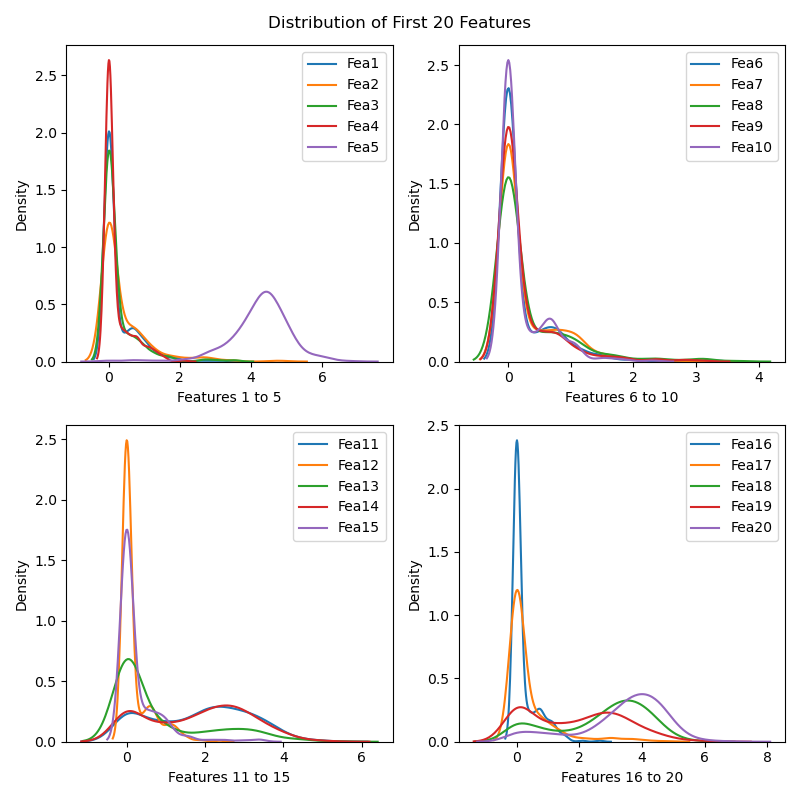
\includegraphics[width=\textwidth]{Q1a_First20Features.png}
        \caption{Density plots for the first 20 features of Dataset A.}
        \label{fig:Q1a_First20Features}
    \end{figure}
    It was decided to show the distribution of five features per plot in order to make the plots more readable. Figure \ref{fig:Q1a_First20Features} shows that all features are positive and of around the same order (i.e. all features are less than 10). Most features seem to be centred around 0, while some features have either a bimodal distribution or are more centered around 3 or 4.

    \item Using \verb|sklearn.decomposition.PCA|, the dataset was reduced to 2 dimensions. The resulting scatter plot is shown in Figure \ref{fig:Q1b_PCA}.
    \begin{figure}[!htb]
        \centering
        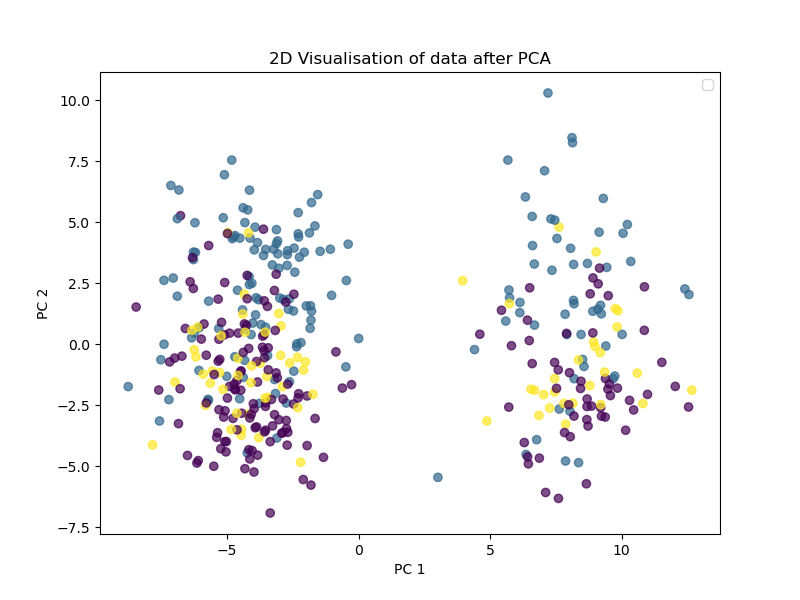
\includegraphics[width=\textwidth]{Q1b_PCA.png}
        \caption{Scatter plot of the first 2 principal components of Dataset A, coloured by label.}
        \label{fig:Q1b_PCA}
    \end{figure}
    Although Figure \ref{fig:Q1b_PCA} shows a linear seperability between two clusters of data, when the points are coloured based on their label, there does not seem to be a clear seperation between the three labels. Referring to what was seen in Figure \ref{fig:Q1a_First20Features}, there were many bimodal features which could explain why there is a clear seperation between the two groups of points in Figure \ref{fig:Q1b_PCA}, but not between the three labels.

    \item After removing the \verb|classification| label (because k-means is an unsupervised method), the data was split into two equally-sized training sets. The \verb|sklearn.cluster.KMeans| method was applied to each training set and predicted the clusters from the complete data. This is possible by creating two k-means models, fitting each model to one of the training sets, and then predicting the clusters of the complete data using each model. This is possible because each training set comes from the same population and so is thought to be representative of the complete dataset. The clusters predicted by each model for the complete dataset is shown in Table \ref{tab:Q1c_contingency}.
    \begin{table}[!htb]
        \centering
        \begin{tabular}{|c||*{8}{c|}|c|}\hline
            \backslashbox{Pred1}{Pred2} & \textbf{0} & \textbf{1} & \textbf{2} & \textbf{3} & \textbf{4} & \textbf{5} & \textbf{6} & \textbf{7} & \textbf{Total} \\
            \hline
            \hline
            \textbf{0} & 0 & 0 & 0 & 0 & 0 & 1 & 0 & 0 & \textbf{1} \\ \hline
            \textbf{1} & 14 & 48 & 0 & 72 & 0 & 69 & 0 & 0 & \textbf{203} \\ \hline
            \textbf{2} & 0 & 0 & 0 & 0 & 6 & 0 & 0 & 22 & \textbf{28} \\ \hline
            \textbf{3} & 0 & 0 & 0 & 0 & 2 & 0 & 0 & 1 & \textbf{3} \\ \hline
            \textbf{4} & 0 & 0 & 0 & 0 & 4 & 0 & 0 & 4 & \textbf{8} \\ \hline
            \textbf{5} & 44 & 9 & 0 & 7 & 0 & 8 & 0 & 0 & \textbf{68} \\ \hline
            \textbf{6} & 0 & 0 & 2 & 0 & 34 & 0 & 3 & 56 & \textbf{95} \\ \hline
            \textbf{7} & 0 & 0 & 0 & 0 & 1 & 0 & 0 & 1 & \textbf{2} \\ \hline
            \hline
            \textbf{Total} & \textbf{58} & \textbf{57} & \textbf{2} & \textbf{79} & \textbf{47} & \textbf{78} & \textbf{3} & \textbf{84} & \textbf{408} \\
            \hline
        \end{tabular}
        \caption{Proportion of data points assigned to each cluster for each model where Pred1 and Pred2 are the two models with default parameters.}
        \label{tab:Q1c_contingency}
    \end{table}

    \item Several of the cluster sizes are too small (i.e. from 1 to 3) which is likely due to there being too many clusters. Because the number of clusters (8, as is default) is too high for this data, the cluster stability is low. In the original dataset, there are three labels. When the same process is repeated with three clusters (instead of eight), the resulting predictions are more consistent with each other, as shown in the contingency table shown in Table \ref{tab:Q1d_contingency}.
    \begin{table}[!htb]
        \centering
        \begin{tabular}{|c||*{4}{c|}|c|}\hline
            \backslashbox{Pred1}{Pred2} & \textbf{0} & \textbf{1} & \textbf{2} & \textbf{Total} \\
            \hline
            \hline
            \textbf{0} & 136 & 0 & 0 & \textbf{136} \\ \hline
            \textbf{1} & 0 & 17 & 90 & \textbf{107} \\ \hline
            \textbf{2} & 0 & 135 & 30 & \textbf{165} \\ \hline
            \hline
            \textbf{Total} & \textbf{136} & \textbf{152} & \textbf{120} & \textbf{408} \\
            \hline
        \end{tabular}
        \caption{Proportion of data points assigned to each cluster for each model where Pred1 and Pred2 are the two models with three clusters.}
        \label{tab:Q1d_contingency}
    \end{table}

    \item To identify the k-means clusters within the PCA figure, the complete dataset was plotted with each point coloured by its cluster. The results of the k-means models with three clusters are shown in Figure \ref{fig:Q1e_PCA}. Comparing this with Figure \ref{fig:Q1b_PCA}, it seems the output of k-means is not consistent with the actual classification of the data.\\
    \begin{figure}[!htb]
        \centering
        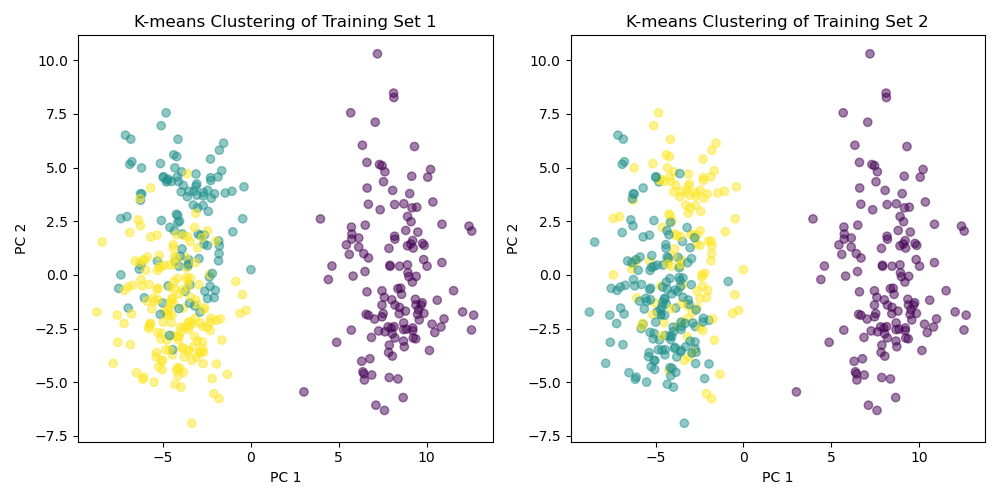
\includegraphics[width=\textwidth]{Q1d_KMeans_3Clusters.png}
        \caption{Scatter plot of the first 2 principal components of Dataset A, coloured by cluster.}
        \label{fig:Q1e_PCA}
    \end{figure}

    To explain the difference between the above process and doing k-means \textit{after} PCA, Figure \ref{fig:Q1e_PCA_KMeans} shows a visualisation of PCA followed by k-means. In general, k-means followed by PCA is better because the clusters are fit on the entire dataset. If PCA is performed first (so that the data is reduced to two dimensions), much of the variance (and therefore information) could have been removed and so the resulting clusters are not representative or accurate. On the other hand, if PCA is performed first to reduce dimensionality while still keeping (for example) 99\% of the variance in the data, then k-means performed on the reduced dataset can outperform k-means performed on the complete dataset. This is because of the curse of dimensionality, where the distance between points in high-dimensional space becomes meaningless.
    \begin{figure}[!htb]
        \centering
        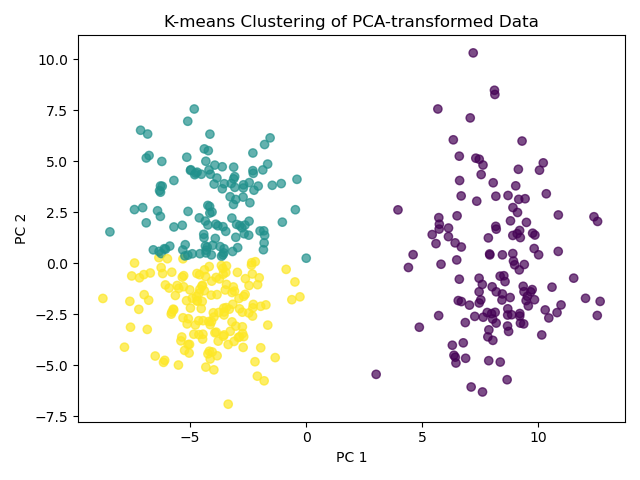
\includegraphics[width=0.7\textwidth]{Q1e_KMeans_after_PCA.png}
        \caption{Scatter plot of the first 2 principal components of Dataset A, coloured by cluster.}
        \label{fig:Q1e_PCA_KMeans}
    \end{figure}
\end{enumerate}

\newpage
\subsection{Dataset B: Missing Labels and Duplicated Observations}
The code used to produce the figures and answer the questions posed in this section are kept in the \verb|src/Q2.ipynb| file.
\begin{enumerate}[label=\alph*)]
    \item Using the \verb|numpy.unique(return_counts=True)| method on the \verb|classification| column of Dataset B, it was found that there are 4 unique labels. The number of observations for each label is shown in Table \ref{tab:Q2a_label_counts}.
    \begin{table}[!htb]
        \centering
        \begin{tabular}{|c|c|c|}\hline
            \textbf{Label} & \textbf{Count} & \textbf{Proportion (\%)} \\ \hline
            1 & 179 & 41.82 \\ \hline
            2 & 157 & 36.68 \\ \hline
            4 & 72 & 16.82 \\ \hline
            \verb|nan| & 20 & 4.67 \\ \hline
        \end{tabular}
        \caption{Number of observations and proportion for each label in Dataset B.}
        \label{tab:Q2a_label_counts}
    \end{table}
    Where the \verb|nan| label indicates a missing value.

    \item Using the \verb|pandas.DataFrame.duplicated()| method, it was found that there were 20 samples that had a duplicate row. The following samples were found to have duplicates:
    \begin{verbatim}
duplicates = {101, 107, 146, 173, 193, 198, 249, 253, 260, 291, 297, 305, 311, 352, 
              359, 382, 389, 396, 409, 424}
    \end{verbatim}
    A strategy to address duplicate observations would be to remove the duplicates from the dataset, so that one instance of each observation remains. This was done with the following code segment:
    \begin{verbatim}
        df.drop_duplicates(subset=df.columns[:-1], inplace=True)
    \end{verbatim}
    Where \verb|df| is the DataFrame containing Dataset B. The \verb|subset| argument specifies to ignore the classifications when identifying duplicates (because some observations may be mislabelled). The \verb|inplace| argument specifies to modify the DataFrame in-place, rather than returning a new DataFrame. The shape of the DataFrame before removing duplicates was \verb|(428, 501)|. There were 20 duplicates, so the shape of the DataFrame after removing duplicates was \verb|(408, 501)|.

    \item Two approaches for handling observations with missing labels are to either remove the observations or to impute the missing labels.\\

    \textbf{Approach 1: Delete Missing Data}\\
    The advantage of this is that it is simple to implement. The disadvantage is that it reduces the size of the dataset, which could lead to a loss of information. Furthermore, if the data is not missing completely at random (i.e. there is some pattern to the missing data), then removing the missing data could introduce bias into the dataset.\\

    \textbf{Approach 2: Impute Missing Data}\\
    The advantage of this is that it preserves the size of the dataset and makes use of all available information. Although it is more complex to implement, if the correct/appropriate choice of imputation method is use, then there could be less bias introduced than removing missing data. The disadvantage is that if an incorrect imputation method is chosen then bias could be introduced and the imputed data could be misleading.\\

    \textbf{MAR and MNAR}\\
    For data that is Missing at Random (MAR) the probability of a value being missing depends on other observed values in the dataset, but not on the missing values themselves.\\

    For data that is Missing Not at Random (MNAR) the probability of a value being missing depends on the missing values themselves.

    \item To predict the missing labels with either multinomial logistic regression or k-nearest neighbours, the data was first split into a training and predicting set, where the training set contains all non-missing data and the predicting set contains all missing data. Using \verb|sklearn.model_selection.GridSearchCV|, the best parameters for each model were found. The results are shown below:
    \begin{verbatim}
    Logistic Regression Best Score: 0.8324009324009325
    Logistic Regression Best Params: {
        'C': 0.0018329807108324356, 'class_weight': 'balanced', 'max_iter': 1000, 
        'penalty': 'l2', 'solver': 'lbfgs'
    }

    KNN Best Score: 0.6882450882450882
    KNN Best Params: {'n_neighbors': 12, 'weights': 'distance'}
    \end{verbatim}
    Where the logistic regression model was run with \verb|multi_class='multinomial'|. Since the logistic regression model performed better, it was used to predict the missing labels. The overall summary of labels is shown in Table \ref{tab:Q2d_label_counts}. The overall proportion of each label is similar before and after imputing missing labels, which suggests that the imputation method does not introduce unexpected bias.
    \begin{table}[!htb]
        \centering
        \begin{tabular}{c||c|c||c|c}
            \textbf{Label} & \textbf{Count Before} & \textbf{Count After} & \textbf{Proportion Before (\%)} & \textbf{Proportion After (\%)} \\ \hline
            1 & 179 & 187 & 43.87 & 43.69 \\ \hline
            2 & 157 & 165 & 38.48 & 38.55 \\ \hline
            4 & 72 & 76 & 17.65 & 17.76 \\
        \end{tabular}
        \caption{Number of observations and proportion for each label in Dataset B before and after imputing missing labels. Missing values are ignored in the calculation of proportions before to allow better comparison.}
        \label{tab:Q2d_label_counts}
    \end{table}
\end{enumerate}

\newpage
\subsection{Dataset C: Missing Data and Outliers}
The code used to produce the figures and answer the questions posed in this section are kept in the \verb|src/Q3.ipynb| file.
\label{subsec:Q3}
\begin{enumerate}[label=\alph*)]
    \item There were missing values found in the following features:
    \begin{verbatim}
    'Fea58', 'Fea142', 'Fea150', 'Fea233', 'Fea269', 'Fea299', 'Fea339','Fea355', 
    'Fea458', 'Fea466', 'Fea491'
    \end{verbatim}
    Where each feature contains 5 missing values. The missing values corresponded to the following rows:
    \begin{verbatim}
    'Sample138', 'Sample143', 'Sample231', 'Sample263', 'Sample389'
    \end{verbatim}
    The missing values were found to be in a $5\times11$ block of data with the rows and features above, which made it more straightforward to impute missing values.

    \item Two methods for imputing missing values across multiple features can be by static imputation or model-based imputation.\\
    
    \textbf{Static Imputation}\\
    An example of this approach is to replace missing values with the mean of available values in the feature. The advantages are that it is easy to implement, fast to compute and easy to interpret. The disadvantages are that it does not take into account the relationships between features, and relationships between features and the target variable and so may introduce bias.\\

    \textbf{Model-Based Imputation}\\
    An example of this approach is to use a regression model to predict the missing values. The advantages are that it takes into account the relationships between features and the target variable, and so may introduce less bias. The disadvantages are that it is more complex to implement, slower to compute and may overfit the data and introduce bias.\\

    \textbf{Multiple Imputation}\\
    Multiple imputation is one of the state-of-the-art techniques that imputes missing values multiple times and then combines the results. The technique is rooted in Bayesian statistics and so imputed values also have a measure of uncertainty attached. The advantages include taking into account relationships between features, and between features and target variables. Furthermore, this method reduces bias and variance introduced as well as providing uncertainty measures. The disadvantages are that it is more complex to implement and slower to compute.

    \item To perform a model-based imputation, the data was split into \verb|X| (data without missing values) and \verb|y| (data with missing values). Each set was then split into \verb|_train| (contains rows without missing values) and \verb|_to_pred| (contains rows with missing values) groups. This was done in order to train the model on the data without missing values and then predict the missing values. Table \ref{tab:Q3c_CV} shows the results of 3-fold cross-validation for several regression models that were tested. The scoring used was the negative root mean squared error so the best model would correspond to the least negative scoring.
    \begin{table}[!htb]
        \centering
        \begin{tabular}{|c|c|c|}\hline
            \textbf{Model} & \textbf{Mean CV Score} & \textbf{Average time (s)} \\ \hline
            Random Forest Regressor & -0.54254 & 4.00 \\ \hline
            Gradient Boosting Regressor & -0.61577 & 11.22 \\ \hline
            KNeighbors Regressor & -0.57284 & 0.06 \\ \hline
            Linear Regression & -1.13666 & 0.50 \\ \hline
            MLP Regressor & -0.94753 & 8.39 \\ \hline
            Support Vector Regressor & -0.56964 & 0.17 \\ \hline
        \end{tabular}
        \caption{Results of 3-fold cross-validation for several regression models. The scoring used was the negative root mean squared error.}
        \label{tab:Q3c_CV}
    \end{table}
    The best model was found to be the Random Forest Regressor, which was then used to predict the missing values. Figure \ref{fig:Q3c_Imputed_Distribution} compares the original and imputed distributions.
    \begin{figure}[!htb]
        \centering
        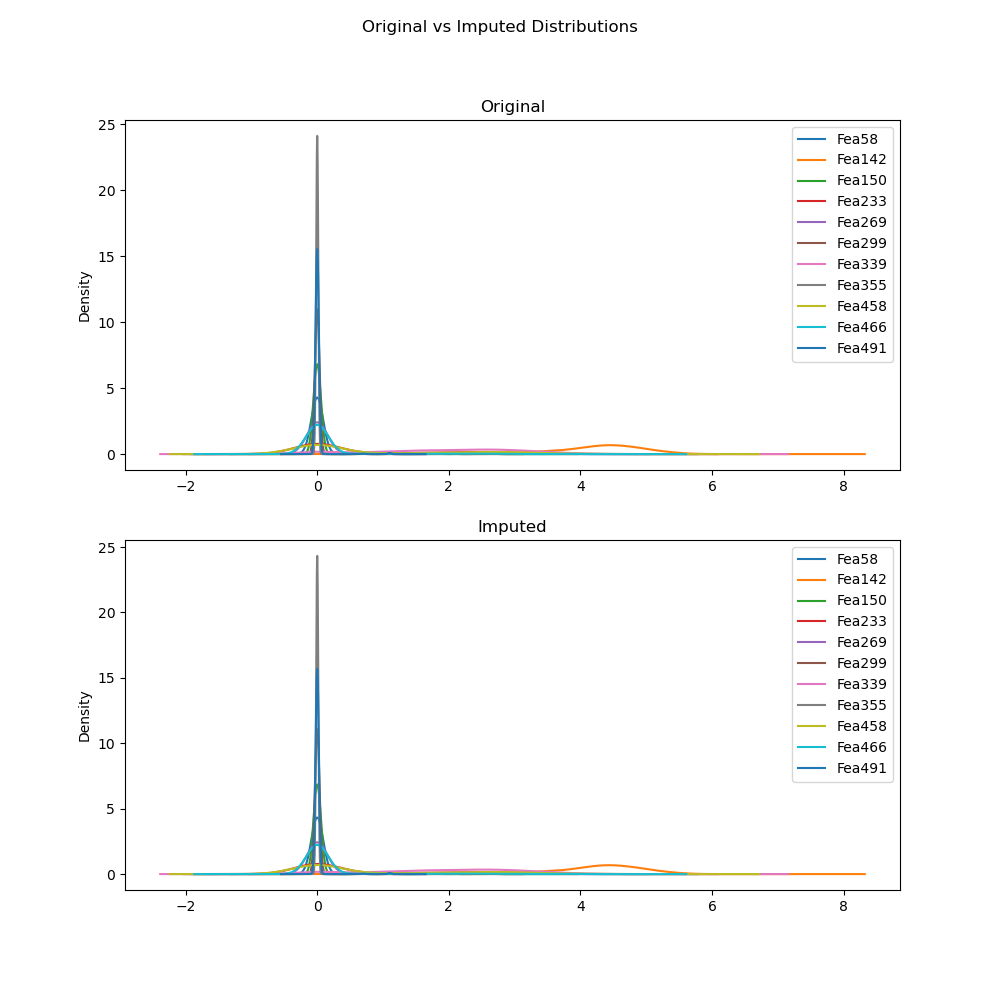
\includegraphics[width=\textwidth]{Q3c_original_vs_imputed_dists.png}
        \caption{Comparison of the original and imputed distributions.}
        \label{fig:Q3c_Imputed_Distribution}
    \end{figure}
    The distributions look very similar, which suggests that the imputation method was successful. %TODO: could include difference table from notebook

    \item The standardisation approach used was to find the $z$-score of each value, which is defined as:
    \begin{equation*}
        z = \frac{x - \mu}{\sigma}
    \end{equation*}
    Where $x$ is a value in a feature, $\mu$ is the mean of the feature and $\sigma$ is the standard deviation of the feature. Typically, values with a $z$-score greater than 3 are considered outliers. Once this filter was applied to the data, it was found that 359 of the 500 features contained at least one outlier and 407 of the 408 sample rows contained at least one outlier. In total, there were 2,659 outliers in the data (1.3\% of the data), and is visualised in Figure \ref{fig:Q3d_outliers}, which shows that there is no discernable pattern to the outliers.
    \begin{figure}[!htb]
        \centering
        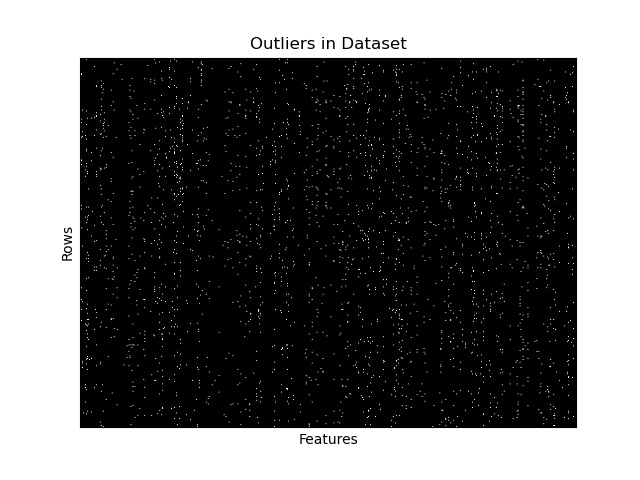
\includegraphics[width=\textwidth]{Q3d_outliers.png}
        \caption{Visualisation of outliers in Dataset C where black means the value is not an outlier and white values indicate an outlier.}
        \label{fig:Q3d_outliers}
    \end{figure}

    \item In order to correct for outlier values, the most straightforward solution was to remove the outlier values and and replace them with a model-based imputation. Although Table \ref{tab:Q3c_CV} shows that the Random Forest Regressor was the best model, it was found that this took too long to impute all values. Similar results were found for the Support Vector Regressor, therefore the KNeighbors Regressor was used to impute the missing values since it was very quick and has a comparable score to those mentioned. Imputing values was done with the \verb|sklearn.impute.IterativeImputer| functionality.
    
    Since there are hundreds of features containing outliers, it was difficult to visualise the distribution of values for each feature with outliers. Instead, the distributions were visualised for the top five features that contained the most outliers. The distirbution of values in the top five features from the original dataset is shown in Figure \ref{fig:Q3e_outliers_original}. For the top four features, the distribution of values could not be found because all values were 0. This is reasonable since Figure \ref{fig:Q3e_outliers_original} shows that the top four features contained mostly zeros, and so outliers were values that were not zero.
    \begin{figure}[!htb]
        \centering
        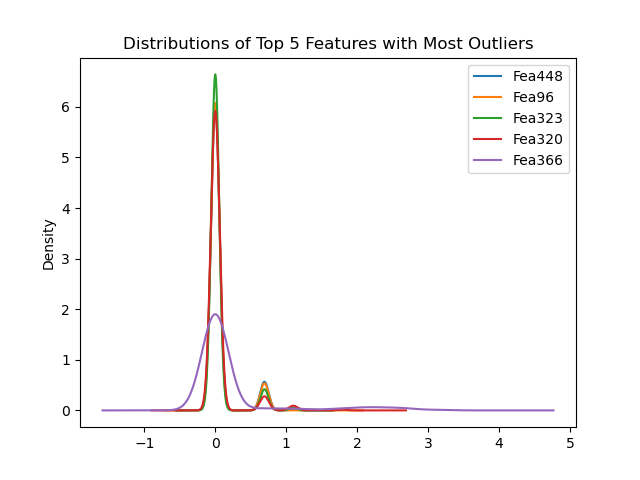
\includegraphics[width=0.7\textwidth]{Q3e_top5_outliers_original.png}
        \caption{Distribution of values in the top five features with the most outliers from the original dataset.}
        \label{fig:Q3e_outliers_original}
    \end{figure}
    The distribution of the fifth feature (\verb|Fea366|) was then plotted from the original and outlier-corrected datasets, and is shown in Figure \ref{fig:Q3e_outliers_corrected}. Similar to the top four features, the imputation also results in many more zero values.
    \begin{figure}[!htb]
        \centering
        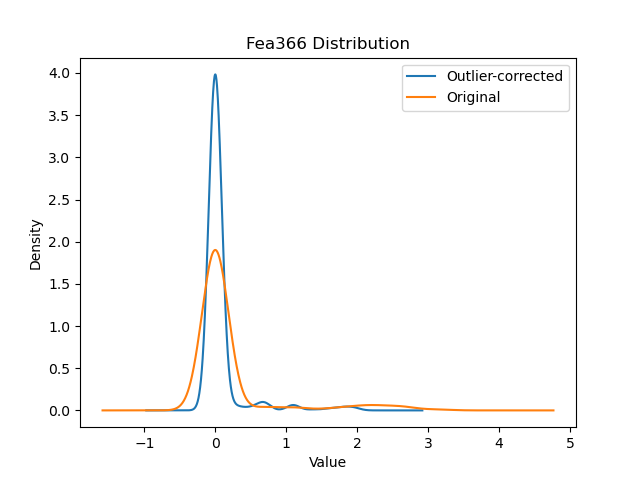
\includegraphics[width=0.7\textwidth]{Q3e_Fea366_dist.png}
        \caption{Distribution of values from Fea366 from the original and outlier-corrected datasets.}
        \label{fig:Q3e_outliers_corrected}
    \end{figure}
\end{enumerate}

\newpage
\section{Section B}
\subsection{Baseline Dataset: Supervised Learning and Random Forests}
The code used to produce the figures and answer the questions posed in this section are kept in the \verb|src/Q4.ipynb| file.
\begin{enumerate}[label=\alph*)]
    \item A decision tree is a non-parametric supervised learning model that uses features to make splits to the data to produce regions that are as pure as possible (i.e. all data points in a region are of the same class).
    
    Bagging (bootstrap aggregating) is a general-purpose technique to reduce the variance of a learning method by training multiple models on different subsets of the data, then combining the results.

    A random forest is an ensemble method that uses bagging to reduce the variance of a decision tree. The difference between bagging and random forests is that random forests consider different subsets of features when making splits in the decision tree. This is done to introduce variability between the trees.

    One criterion to measure the quality of a split is the Gini impurity, which is defined as:
    \begin{equation*}
        G(Q_m)=1-\sum_{k=1}^{K}p_{mk}^2
    \end{equation*}
    where $K$ is the number of classes, $Q_m$ is the region of data at node $m$ with $n_m$ samples and $p_{mk}$ is the proportion of training samples in region $m$ that are of class $k$:
    \begin{equation*}
        p_{mk}=\frac{1}{n_m}\sum_{x_i\in Q_m}I(y_i=k)
    \end{equation*}
    where $I$ is the indicator function.\\
    The Gini impurity is a measure of purity of a node ranging between 0 and 0.5, where 0 means that all the samples at the node are of the same class and 0.5 means that the samples are equally distributed amongst different classes.

    Two hyperparameters of a single tree within a random forest are the maximum depth of the tree and maximum number of features to consider when performing a split. A heuristic to determine the value of \verb|max_features| to use for a model is by taking the square root of the total number of features.

    \item To pre-process the data for a random forest model, the data was checked for missing values, duplicate rows and outliers. It was decided that scaling was not needed since it is not necessary for decision trees or random forests. There were 6,689 outliers found (1.34\% of data), which were corrected using the same method described in Section \ref{subsec:Q3}. Figure \ref{fig:Q4b_outliers} shows the distribution of outliers in the data.
    \begin{figure}[!htb]
        \centering
        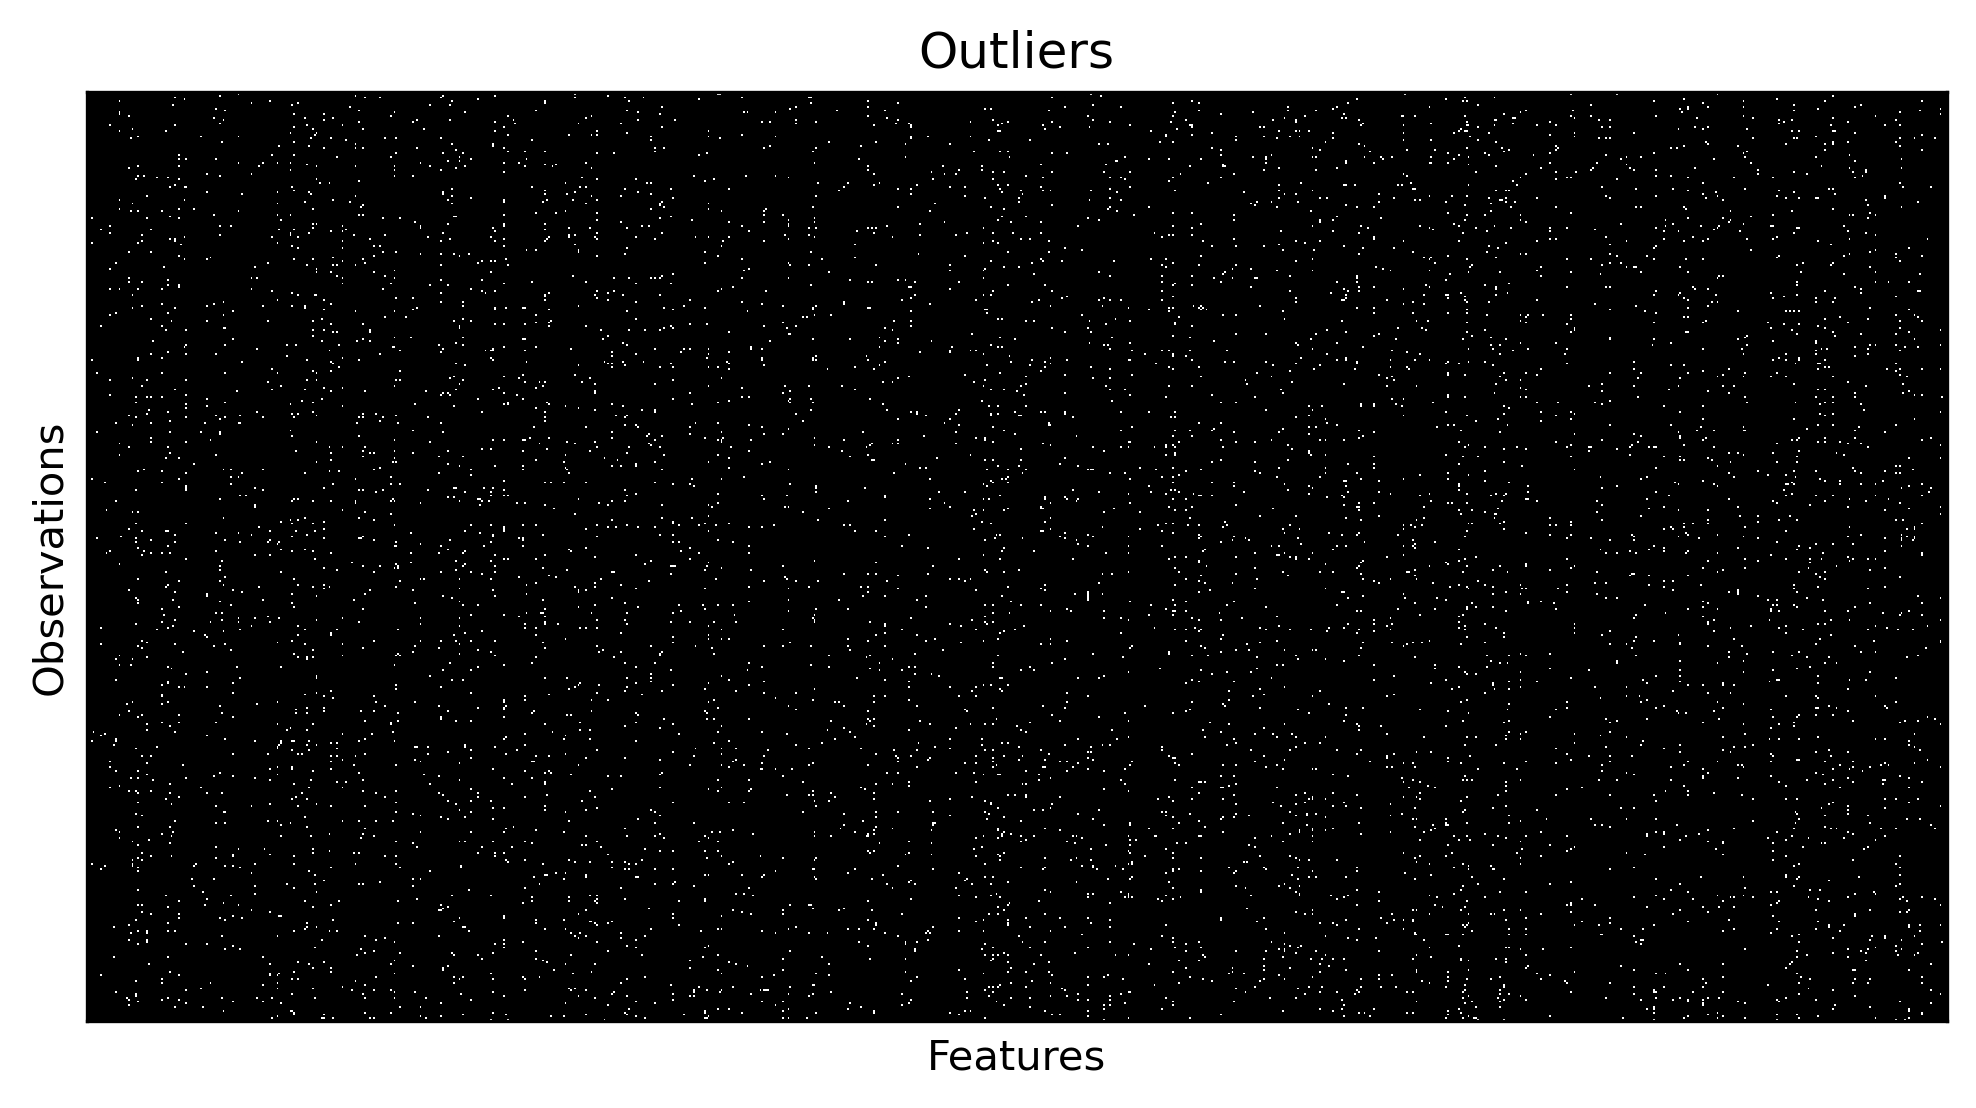
\includegraphics[width=\textwidth]{Q4b_outliers.png}
        \caption{Visualisation of outliers in the baseline dataset where black means the value is not an outlier and white values indicate an outlier.}
        \label{fig:Q4b_outliers}
    \end{figure}

    To prevent data leakage (where information from the test set is somehow incorporated into the training stage), the data was split into a training and test set. Independently, outliers were found within each set and replaced with \verb|np.nan| values. There were 5,261 outliers found in the training set and 1,276 outliers found in the test set. In total, there were fewer outliers found than in the original (complete) dataset, which is thought to be because the mean and standard deviation values would be different and so the $z$-scores would be different.

    Next, the missing values were imputed using the KNeighbors Regressor, since it was found to be effective and quick in Section \ref{subsec:Q3}. The model was trained on the training set and then used to predict the missing values in the training and test sets. Once the outliers were corrected, the pre-processing stage was complete.

    \item The Random Forest Classifier was then trained on the training set with default parameters, and labels were predicted from the test set. The accuracy was found to be 0.97. Further evaluation metrics used were precision, recall and f1-score which are shown in Table \ref{tab:Q4c_metrics}. The confusion matrix was also found and is shown in Table \ref{tab:Q4c_confusion_matrix}.
    \begin{table}[!htb]
        \centering
        \begin{tabular}{|c|c|c|c|}\hline
            \textbf{Label} & \textbf{Precision} & \textbf{Recall} & \textbf{F1-Score} \\ \hline
            1 & 0.93 & 1.00 & 0.96 \\ \hline
            2 & 1.00 & 1.00 & 1.00 \\ \hline
            3 & 1.00 & 0.88 & 0.94 \\ \hline
        \end{tabular}
        \caption{Evaluation metrics for the Random Forest Classifier.}
        \label{tab:Q4c_metrics}
    \end{table}
    \begin{table}[!htb]
        \centering
        \begin{tabular}{|c||*{3}{c|}|c|}\hline
            \backslashbox{True}{Pred} & \textbf{1} & \textbf{2} & \textbf{3} & \textbf{Total} \\
            \hline
            \hline
            \textbf{1} & 38 & 0 & 0 & \textbf{38} \\ \hline
            \textbf{2} & 0 & 36 & 0 & \textbf{36} \\ \hline
            \textbf{3} & 3 & 0 & 23 & \textbf{26} \\ \hline
            \hline
            \textbf{Total} & \textbf{41} & \textbf{36} & \textbf{23} & \textbf{100} \\
            \hline
        \end{tabular}
        \caption{Confusion matrix for the Random Forest Classifier.}
        \label{tab:Q4c_confusion_matrix}
    \end{table}

    \item In order to optimise the model with respect to the number of trees in the random forest, a validation curve was plotted, which shows the validation score (accuracy) for different values of the hyperparameter. Although the question outlined that we "should be able to do this without explicilty performing cross-validation", it was decided that the validation curve \textit{implicilty} performs cross-validation and so is acceptable. There was no way to fine-tune the model hyperparameter without performing some sort of cross-validation. The validation curve is shown in Figure \ref{fig:Q4d_validation_curve}.
    \begin{figure}[!htb]
        \centering
        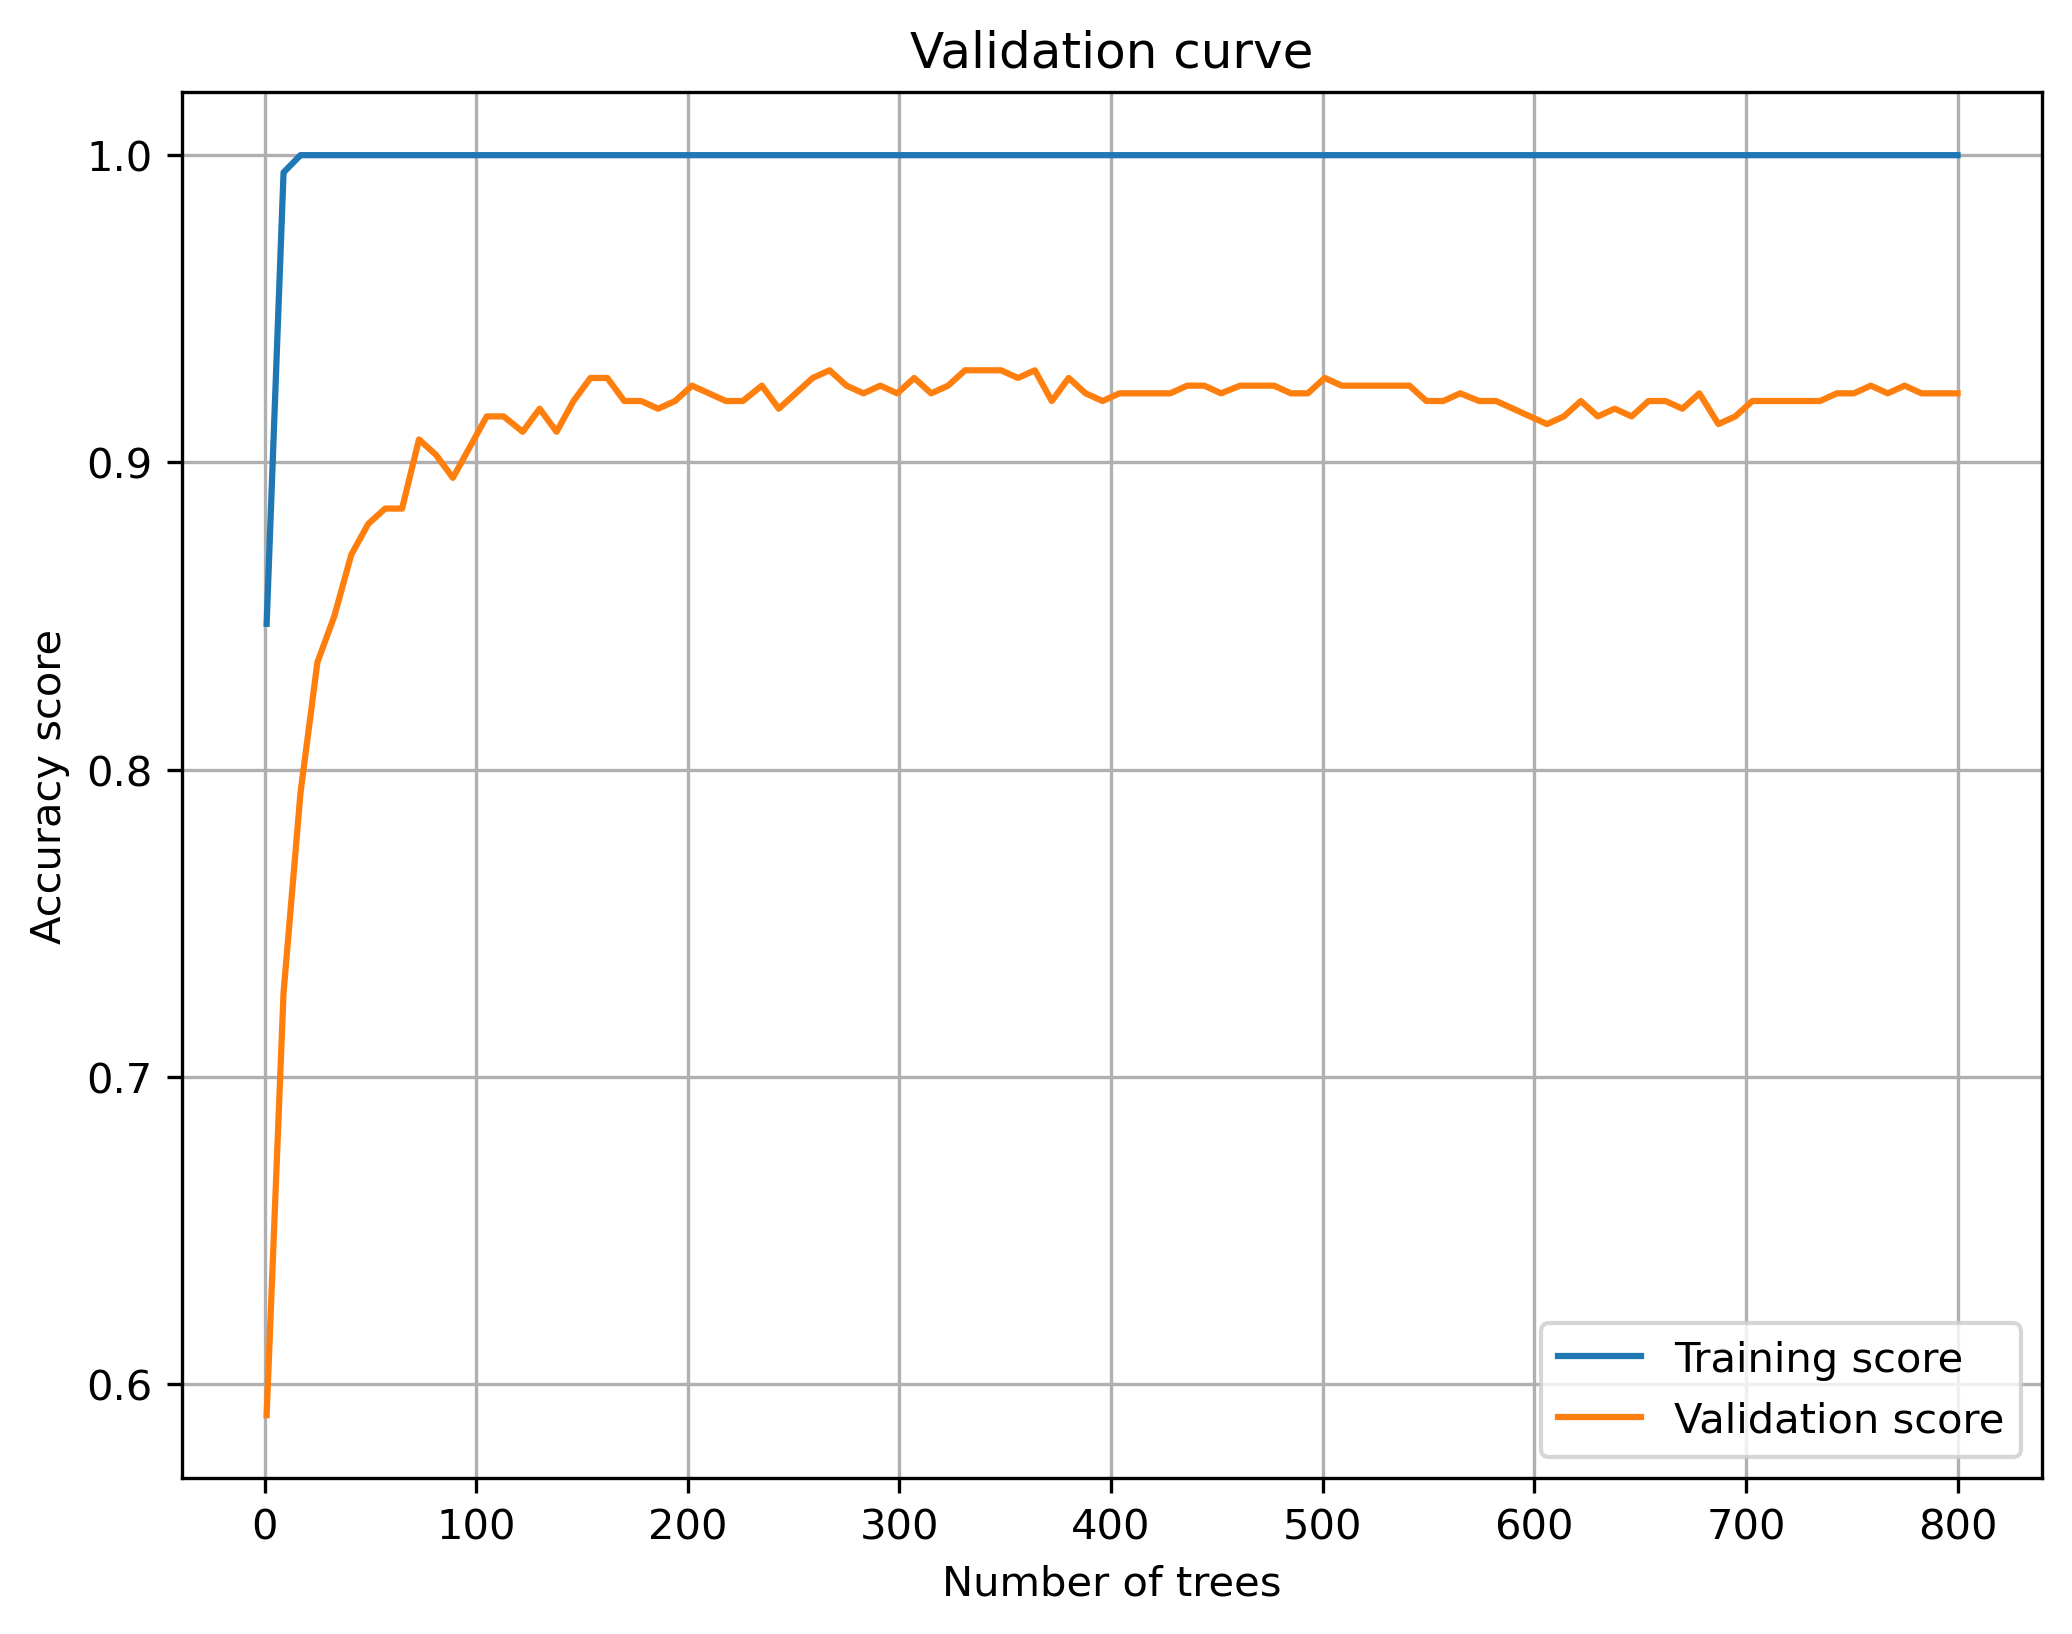
\includegraphics[width=0.8\textwidth]{Q4d_validation_curve.png}
        \caption{Validation curve for the Random Forest Classifier with respect to the number of trees.}
        \label{fig:Q4d_validation_curve}
    \end{figure}
    The validation curve shows a peak in accuracy at approximately 300 trees, after which the accuracy looks to decrease. Therefore, it was decided to use 300 trees for the final model.

    \item The \verb|sklearn.ensemble.RandomForestClassifier| model is able to return the feature importances, which are calculated by the mean decrease in Gini impurity of each feature (which is a value between 0 and 1, and the sum of all values sum to 1). Therefore, the most important feature is the one with the highest mean decrease in Gini impurity. It was decided to find the top features that contribute to 90\% of the total feature importance, in other words the cumulative sum of the feature importances is 0.9. Using this heuristic, it was found that the top 268 features sum to 0.9003 and so the top 268 features were used (originally, there were 1,000 features).
    
    A new Random Forest Classifier was then trained on the subset of the training set containing the top 268 importance features, with 300 trees. In parallel, a Random Forest Classifier was trained on the entire training set with 300 trees. The accuracy of the original (i.e. with 1,000 features) model was 0.94, and the retrained model (with 268 features) had an accuracy of 0.94 also. The confusion matrices for each of these models are shown in Tables \ref{tab:Q4e_confusion_matrix_original} and \ref{tab:Q4e_confusion_matrix_retrained} respectively.
    \begin{table}[!htb]
        \centering
        \begin{tabular}{|c||*{3}{c|}|c|}\hline
            \backslashbox{True}{Pred} & \textbf{1} & \textbf{2} & \textbf{3} & \textbf{Total} \\
            \hline
            \hline
            \textbf{1} & 38 & 0 & 0 & \textbf{38} \\ \hline
            \textbf{2} & 0 & 36 & 0 & \textbf{36} \\ \hline
            \textbf{3} & 6 & 0 & 20 & \textbf{26} \\ \hline
            \hline
            \textbf{Total} & \textbf{44} & \textbf{36} & \textbf{20} & \textbf{100} \\
            \hline
        \end{tabular}
        \caption{Confusion matrix for the Random Forest Classifier with 1,000 features.}
        \label{tab:Q4e_confusion_matrix_original}
    \end{table} 
    \begin{table}[!htb]
        \centering
        \begin{tabular}{|c||*{3}{c|}|c|}\hline
            \backslashbox{True}{Pred} & \textbf{1} & \textbf{2} & \textbf{3} & \textbf{Total} \\
            \hline
            \hline
            \textbf{1} & 37 & 0 & 1 & \textbf{38} \\ \hline
            \textbf{2} & 1 & 35 & 0 & \textbf{36} \\ \hline
            \textbf{3} & 4 & 0 & 22 & \textbf{26} \\ \hline
            \hline
            \textbf{Total} & \textbf{42} & \textbf{35} & \textbf{23} & \textbf{100} \\
            \hline
        \end{tabular}
        \caption{Confusion matrix for the Random Forest Classifier with 268 features.}
        \label{tab:Q4e_confusion_matrix_retrained}
    \end{table}
    The accuracies of the two models are similar, which suggests that the 268 features are sufficient to produce a model with similar performance to the original model which uses all available data. This is useful because it means that the model can be trained on a subset of the data, which is faster and requires less memory.

    \item To repeat steps (b), (c) and (e), it was decided to use the Support Vector Classifier (SVC). Initially, the Gradient Boosting Classifier was to be used, however it was decided to steer away from decision trees altogehter.
    
    Since the SVC is much more sensitive to the scale of data than random forests, the pre-processing stage was modified to include scaling. The same (outlier-corrected) training and test sets were used. A standard scaler was then fit to the training set and used to transform the training and test sets. The SVC was then trained on the training set with default parameters and labels were predicted from the test set. The accuracy was found to be 0.89. The precision, recall and f1-score values are shown in Table \ref{tab:Q4f_metrics}. The confusion matrix was also found and is shown in Table \ref{tab:Q4f_confusion_matrix}.
    \begin{table}[!htb]
        \centering
        \begin{tabular}{|c|c|c|c|}\hline
            \textbf{Label} & \textbf{Precision} & \textbf{Recall} & \textbf{F1-Score} \\ \hline
            1 & 0.82 & 0.97 & 0.89 \\ \hline
            2 & 1.00 & 0.81 & 0.89 \\ \hline
            3 & 0.88 & 0.88 & 0.88 \\ \hline
        \end{tabular}
        \caption{Evaluation metrics for the Support Vector Classifier with default parameters.}
        \label{tab:Q4f_metrics}
    \end{table}
    \begin{table}[!htb]
        \centering
        \begin{tabular}{|c||*{3}{c|}|c|}\hline
            \backslashbox{True}{Pred} & \textbf{1} & \textbf{2} & \textbf{3} & \textbf{Total} \\
            \hline
            \hline
            \textbf{1} & 37 & 0 & 1 & \textbf{38} \\ \hline
            \textbf{2} & 5 & 29 & 2 & \textbf{36} \\ \hline
            \textbf{3} & 3 & 0 & 23 & \textbf{26} \\ \hline
            \hline
            \textbf{Total} & \textbf{45} & \textbf{29} & \textbf{26} & \textbf{100} \\
            \hline
        \end{tabular}
        \caption{Confusion matrix for the Support Vector Classifier.}
        \label{tab:Q4f_confusion_matrix}
    \end{table}

    The \verb|sklearn.inspection.permutation_importance| method was then used to calculate a measure for the feature importances. These are defined as the decrease in a model score when a single feature value is randomly shuffled, and so can be thought of as weights to each feature. Therefore, the most important features are those with positive values (i.e. the model score decreases when the feature value is randomly shuffled). The top 208 features were found to have positive values, and so were used for the final model. The accuracy of the model with all features was 0.89, while the accuracy of the model with 208 features was 0.88. The confusion matrices for each of these models are shown in Tables \ref{tab:Q4f_confusion_matrix_original} and \ref{tab:Q4f_confusion_matrix_retrained} respectively.
    \begin{table}[!htb]
        \centering
        \begin{tabular}{|c||*{3}{c|}|c|}\hline
            \backslashbox{True}{Pred} & \textbf{1} & \textbf{2} & \textbf{3} & \textbf{Total} \\
            \hline
            \hline
            \textbf{1} & 37 & 0 & 1 & \textbf{38} \\ \hline
            \textbf{2} & 5 & 29 & 2 & \textbf{36} \\ \hline
            \textbf{3} & 3 & 0 & 23 & \textbf{26} \\ \hline
            \hline
            \textbf{Total} & \textbf{45} & \textbf{29} & \textbf{26} & \textbf{100} \\
            \hline
        \end{tabular}
        \caption{Confusion matrix for the Support Vector Classifier with 1,000 features and default parameters.}
        \label{tab:Q4f_confusion_matrix_original}
    \end{table}
    \begin{table}[!htb]
        \centering
        \begin{tabular}{|c||*{3}{c|}|c|}\hline
            \backslashbox{True}{Pred} & \textbf{1} & \textbf{2} & \textbf{3} & \textbf{Total} \\
            \hline
            \hline
            \textbf{1} & 37 & 1 & 0 & \textbf{38} \\ \hline
            \textbf{2} & 3 & 33 & 0 & \textbf{36} \\ \hline
            \textbf{3} & 7 & 1 & 18 & \textbf{26} \\ \hline
            \hline
            \textbf{Total} & \textbf{47} & \textbf{35} & \textbf{18} & \textbf{100} \\
            \hline
        \end{tabular}
        \caption{Confusion matrix for the Support Vector Classifier with 208 features and default parameters.}
        \label{tab:Q4f_confusion_matrix_retrained}
    \end{table}

    The accuracy of the model with 208 features is slightly lower than the model with 1,000 features, which suggests that the 208 features are not sufficient to produce a model with similar performance to the original model which uses all available data. This may be because a support vector machine's performance depends on the support vectors in the data, instead of entire features themselves. Therefore, it is possible that the 208 features do not contain all the support vectors present in the complete dataset.

    In general, the SVC seemed to perform worse than the random forest classifier. This could be due a number of reasons:
    \begin{itemize}
        \item The SVC is more sensitive to the scale of the data and so the data may have been scaled incorrectly.
        \item The SVC is more sensitive to outliers and so the outliers may not have been corrected or identified properly.
        \item The SVC model was not hyperparameter tuned and so may not have been optimised.
        \item The dataset may be more suitable for a random forest classifier than a support vector classifier.
    \end{itemize}
\end{enumerate}

\newpage
\subsection{Baseline Dataset: Unsupervised Learning - Clustering}
The code used to produce the figures and answer the questions posed in this section are kept in the \verb|src/Q5.ipynb| file.
\begin{enumerate}[label=\alph*)]
    \item The two clustering techniques used were $k$-means and agglomerative clustering. The $k$-means algorithm aims to partition the observations into $k$ clusters in which each observations belongs to the cluster with the nearest mean. The agglomerative clustering algorithm aims to build a hierarchy of clusters by iteratively merging the two closest clusters until some stopping criterion is satisfied (e.g. $k$ clusters are found). The difference between the two algorithms is that $k$-means is a partitioning algorithm, whereas agglomerative clustering is a hierarchical algorithm.
    
    Before agglomerative, spectral and density-based clustering were attempted, however, these were not successful. Spectral clustering failed due to there being features in the dataset with all values equal to zero, which resulted in a non-fully-connected graph. Density-based clustering proved to be too difficult to optimise parameters (e.g. the minimum number of samples in a cluster and epsilon) and so was not used.

    Both $k$-means and agglomerative clustering require a number of clusters to be passed to it. The optimum number of clusters was found by calculating the silhouette score for different values of $k$. The silhouette score is a measure of how similar an observation is to its own cluster compared to other clusters. The silhouette score is defined as the mean of all silhouette coefficients, where the silhouette coefficient for a single observation is defined as:
    \begin{equation*}
        s_i=\frac{b_i-a_i}{\max(a_i,b_i)}
    \end{equation*}
    Where $a_i$ is the mean distance between point $i$ and all other points in the same cluster, and $b_i$ is the mean distance between point $i$ and all other points in the next nearest cluster. The optimal number of clusters is the one that maximises the silhouette score. The silhouette scores for $k$-means and agglomerative clustering are shown in Figures \ref{fig:Q5a_silhouette_scores} and \ref{fig:Q5a_silhouette_scores_agg} respectively.
    \begin{figure}[!htb]
        \centering
        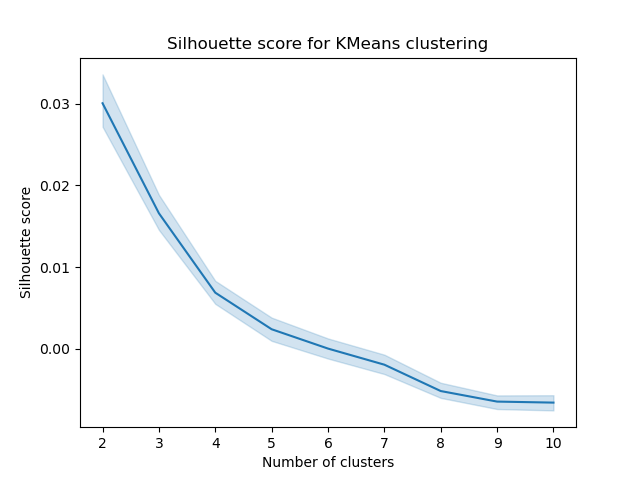
\includegraphics[width=0.8\textwidth]{Q5a_KMeans_silhouette.png}
        \caption{Silhouette scores for $k$-means clustering.}
        \label{fig:Q5a_silhouette_scores}
    \end{figure}
    \begin{figure}[!htb]
        \centering
        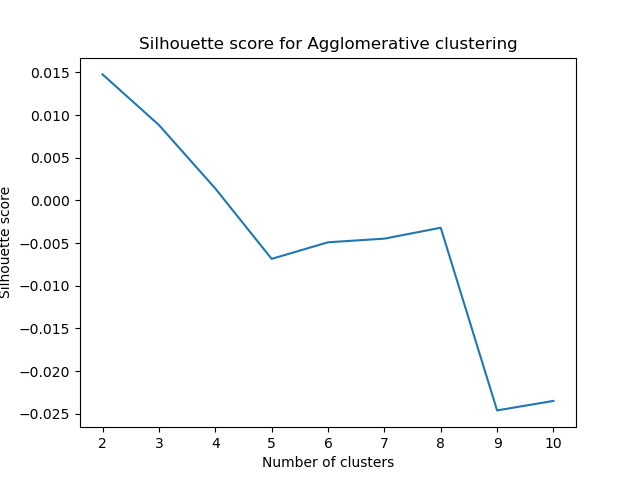
\includegraphics[width=0.8\textwidth]{Q5a_Agglomerative_silhouette.png}
        \caption{Silhouette scores for agglomerative clustering.}
        \label{fig:Q5a_silhouette_scores_agg}
    \end{figure}

    It was found that both clustering algorithms maximised their silhouette scores when $k=2$. Then, both $k$-means and agglomerative clustering were trained on the entire dataset (no test set since these are unsupervised learning algorithms) with $k=2$. The contingency table to summarise the number of observations assigned to each cluster using each technique is shown in Table \ref{tab:Q5a_contingency_table}.
    \begin{table}[!htb]
        \centering
        \begin{tabular}{|c||*{2}{c|}|c|}\hline
            \backslashbox{$k$-means}{Aggl.} & \textbf{0} & \textbf{1} & \textbf{Total} \\
            \hline
            \hline
            \textbf{0} & 156 & 73 & \textbf{229} \\ \hline
            \textbf{1} & 119 & 152 & \textbf{271} \\ \hline
            \hline
            \textbf{Total} & \textbf{275} & \textbf{225} & 500 \\
            \hline
        \end{tabular}
        \caption{Contingency table for $k$-means and agglomerative clustering.}
        \label{tab:Q5a_contingency_table}
    \end{table}

    \item To determine the most discriminative features, a Random Forest Classifier was training on the entire dataset with default parameters where the labels were the cluster assignments from each clustering technique used. Two random forest classifier were trained, one for the labels from each technique. The most importance features were determined to be those that contribute to 99\% of the total feature importance. For $k$-means, this was found to be the top 562 features, and for agglomerative clustering, this was found to be the top 604 features. Two subsets of the data were then created, one suited for each clustering technique and the clustering models were trained again. Tables \ref{tab:Q5b_kmeans_contingency_table} and \ref{tab:Q5b_agg_contingency_table} show the contingency tables for $k$-means and agglomerative clustering respectively comparing the models trained on the complete and subset of the dataset.
    \begin{table}[!htb]
        \centering
        \begin{tabular}{|c||*{2}{c|}|c|}\hline
            \backslashbox{Total}{Subset} & \textbf{0} & \textbf{1} & \textbf{Total} \\
            \hline
            \hline
            \textbf{0} & 229 & 0 & \textbf{229} \\ \hline
            \textbf{1} & 1 & 270 & \textbf{271} \\ \hline
            \hline
            \textbf{Total} & \textbf{230} & \textbf{270} & 500 \\
            \hline
        \end{tabular}
        \caption{Contingency table for $k$-means clustering with the complete and subset of the dataset.}
        \label{tab:Q5b_kmeans_contingency_table}
    \end{table}
    \begin{table}[!htb]
        \centering
        \begin{tabular}{|c||*{2}{c|}|c|}\hline
            \backslashbox{Total}{Subset} & \textbf{0} & \textbf{1} & \textbf{Total} \\
            \hline
            \hline
            \textbf{0} & 259 & 16 & \textbf{275} \\ \hline
            \textbf{1} & 38 & 187 & \textbf{225} \\ \hline
            \hline
            \textbf{Total} & \textbf{297} & \textbf{203} & 500 \\
            \hline
        \end{tabular}
        \caption{Contingency table for agglomerative clustering with the complete and subset of the dataset.}
        \label{tab:Q5b_agg_contingency_table}
    \end{table}

    It was found that the $k$-means clustering model trained on the subset of data achieved an almost equivalent result to the model trained on the complete dataset. However, the agglomerative clustering model trained on the subset of data performed more differently than the model trained on the complete dataset. This suggests that the agglomerative clustering model is more sensitive to the number of features used than the $k$-means clustering model.

    \item To visualise the clusters in a lower-dimensional space coloured by certain characteristics, it was decided to use the cluster labels produced from the most recent models (i.e. those trained on subsets of the data). Principal Component Analysis (PCA) was used to reduce the dimensionality of the data to two dimensions. The points coloured by cluster membership for both models is shown in Figure \ref{fig:Q5c_clusters}.
    \begin{figure}[!htb]
        \centering
        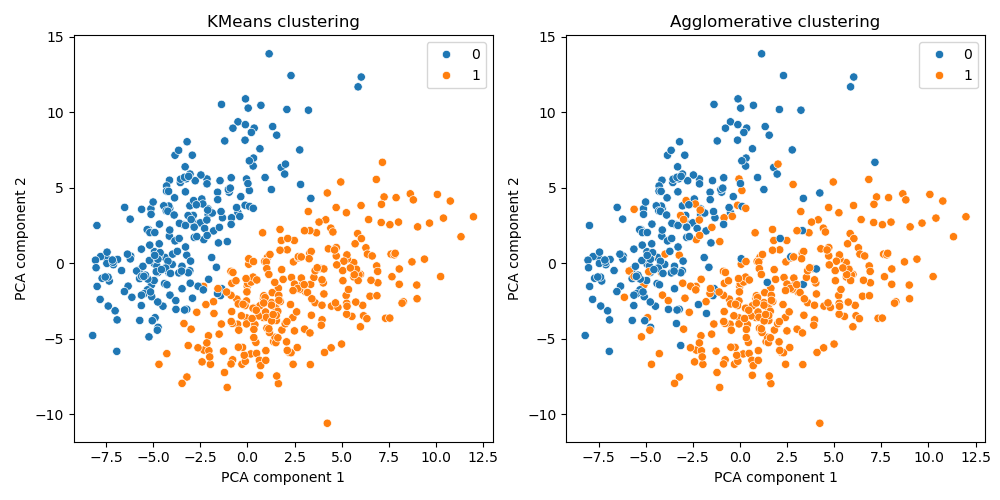
\includegraphics[width=\textwidth]{Q5c_KMeans_Agglomerative_PCA.png}
        \caption{Clusters coloured by cluster membership for $k$-means and agglomerative clustering models.}
        \label{fig:Q5c_clusters}
    \end{figure}
    The $k$-means clustering model seems to have produced two clusters that are well separated, whereas the agglomerative clustering model seems to have produced two clusters that are not as well separated. This is consistent with the contingency tables shown in Tables \ref{tab:Q5b_kmeans_contingency_table} and \ref{tab:Q5b_agg_contingency_table}.

    The data was then coloured by the values of the most and next most discriminative features, for each model. These are shown in Figures \ref{fig:Q5c_top_feature} and \ref{fig:Q5c_next_feature} respectively.
    \begin{figure}[!htb]
        \centering
        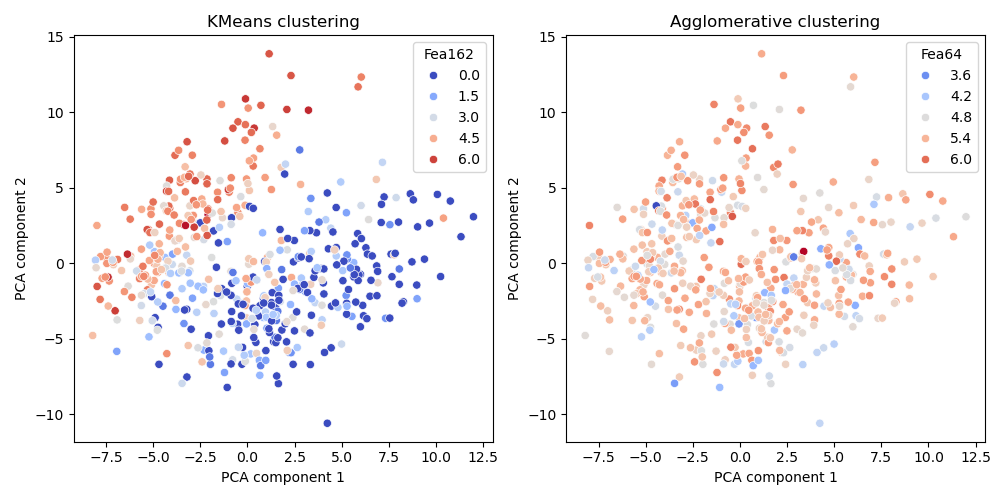
\includegraphics[width=\textwidth]{Q5c_KMeans_Agglomerative_PCA_top_feature.png}
        \caption{Clusters coloured by the most discriminative feature for $k$-means and agglomerative clustering models.}
        \label{fig:Q5c_top_feature}
    \end{figure}
    \begin{figure}[!htb]
        \centering
        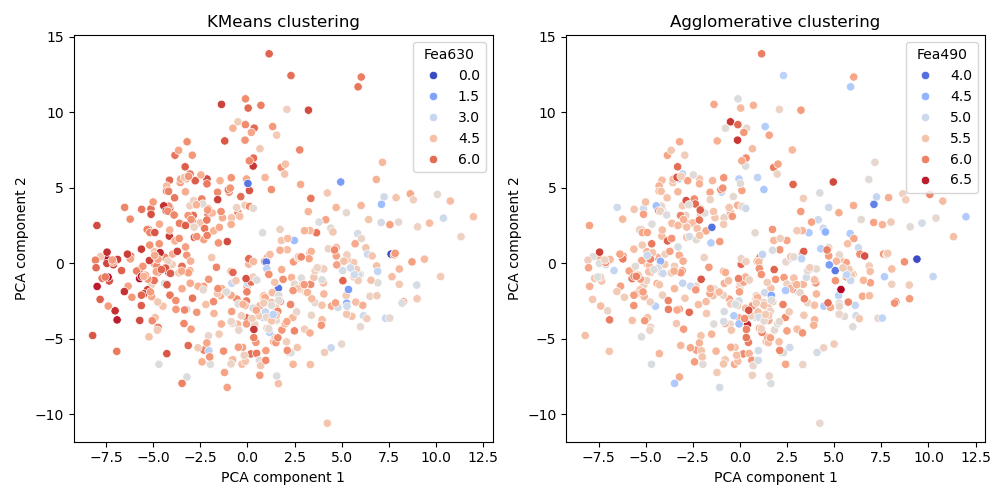
\includegraphics[width=\textwidth]{Q5c_KMeans_Agglomerative_PCA_second_feature.png}
        \caption{Clusters coloured by the next most discriminative feature for $k$-means and agglomerative clustering models.}
        \label{fig:Q5c_next_feature}
    \end{figure}
    Figure \ref{fig:Q5c_top_feature} shows that the most discriminative feature for $k$-means clustering is able to separate the clusters well, whereas the most discriminative feature for agglomerative clustering is not able to separate the clusters well. Figure \ref{fig:Q5c_next_feature} shows that the next most discriminative feature for $k$-means does separate the clusters as well as the most discriminative feature, however still separates the clusters more so than the second most important feature for agglomerative clustering. These Figures seem to indicate that agglomerative clustering does not depend on the most discriminative features as much as $k$-means clustering does, which suggest that the entire dataset is best to be used for agglomerative clustering.
\end{enumerate}

\newpage
\section{Appendix}
\subsection{README}
\textbf{S1: Applied Data Science - Coursework}\\
This repository is for the submission of the M1 Applied Data Science Module as part of the MPhil in Data Intensive Science at the University of Cambridge. The task was to provide solutions to the problems set out in the coursework instructions \verb|DIS_MPhil_M1_Coursework.pdf|.\\

\textbf{Installation}\\
To install the required packages into a new conda environment, run the following command in the root directory:
\begin{verbatim}
    $ conda env create -f environment.yml
\end{verbatim}
To activate the environment, run the following command in the root directory:
\begin{verbatim}
    $ conda activate cambridge
\end{verbatim}

\textbf{Usage}\\
It was decided to use \verb|.ipynb| files for the coursework, as this allows for the inclusion of code, plots, and text in a single document. To run the code from the command line, run the following command in the root directory:
\begin{verbatim}
    $ jupyter execute src/Qx.ipynb
\end{verbatim}
Where `x` is the question number (1-5), so to run the code for question 1, run the following command:
\begin{verbatim}
    $ jupyter execute src/Q1.ipynb 
\end{verbatim}
Alternatively, the code can be run in the browser with the following command:
\begin{verbatim}
    $ jupyter notebook src/Qx.ipynb 
\end{verbatim}

\textbf{Expected Runtime}\\
The code was developed on a 2019 MacBook Pro with a 2.4 GHz 8-Core Intel Core i9 processor and 32 GB of RAM. The runtime for each question is was found to be as follows:
\begin{itemize}
    \item Q1: 12 seconds
    \item Q2: 11 seconds (around 10 minutes with empty \verb|Data/pickles| folder)
    \item Q3: 1 minute 45 seconds
    \item Q4: 3 minutes 20 seconds
    \item Q5: 1 minute 5 seconds
\end{itemize}

\textbf{Use of AI}\\
GitHub copilot was used in auto-completion for basic functionality code. The use of AI was not used for idea generation, proofreading, optimisation, or any other task.\\

\textbf{Support}\\
For any questions or issues, please contact me at \verb|dp702@cam.ac.uk|.


\end{document}